\documentclass{article}

\usepackage[left=2.5cm, right=2.5cm, top=2.5cm, bottom=2.5cm]{geometry}
\usepackage{graphicx}
\usepackage{physics}
\usepackage{subcaption}
\usepackage{hyperref}
\usepackage[version=4]{mhchem}


\title{Exercise 3, TFY4235 Computational physics}
\author{Martin Johnsrud}
\vspace{-8ex}
\date{}


\begin{document}
    \maketitle
    \section*{Introduction}
        This is an implementation of \cite{exercise}.
    \section*{Theory and implementation}
    The diffusion equation, can be written as
    \begin{equation*}
        \Delta t \pdv{t} C(z, t) = \Delta t \left(K(z) \pdv[2]{z} + \dv{K(z)}{z}\pdv{z}\right) C(z, t) = \mathcal{D} C(z, t).
    \end{equation*}
    Discretizing the spatial part, and applying boundary conditions, gives
    \begin{equation*}
        \Delta t \pdv{t} C_n(t) = \mathcal{D}_{nm} C_n(t) + S_n(t),
    \end{equation*}
    where 
    \begin{align*}
        \mathcal{D} &=
        \begin{pmatrix}
            -4\alpha K_0 - 2\Gamma & 4\alpha K_0 & 0 & \dots&0 \\
            -\frac{\alpha}{2} K_1' + 2\alpha K_1 & -4 \alpha K_1 & \frac{\alpha}{2}K_1' + 2\alpha K_1 &  \dots & 0 \\
            0 & \ddots & \ddots & \ddots & 0\\
            0 & \dots &-\frac{\alpha}{2} K_{N-1}' + 2\alpha K_{N-1} & -4 \alpha K_{N-1} & \frac{\alpha}{2}K_{N-1}' + 2\alpha K_{N-1} \\
             0 & \dots & 0 & 4\alpha K_N & -4\alpha K_N
        \end{pmatrix},\\
        S(t) & =  
        \begin{pmatrix}
            2\Gamma C_\mathrm{eq}(t) &0&\dots&0
        \end{pmatrix}^T \quad 
    \Gamma = 2 \frac{\alpha k_w \Delta z}{K_0} \left(K_0 - \frac{1}{2}(-\frac{3}{2} K_0 + 2K_1 - \frac{1}{2}K_2)\right), \quad
     \alpha = \frac{\Delta t}{2 \Delta z^2 },\\
      K_n' & = K_{n+1} - K_{n-1}
    \end{align*}
    The Chranck-Nichelson scheme then yields
    \begin{equation*}
        C_n^{i+1}  = C_n^i + \frac{1}{2} (\mathcal{D}_{nm} C_m^i + S_n^i) + \frac{1}{2} (\mathcal{D}_{nm} C_m^{i+1} + S_n^{i+1}),
    \end{equation*}
    so the equatino to be solved to get the next timestep is
    \begin{equation*}
        A_{nm} C_{m}^{i+1} = V_n^i, \quad V_n^i = \left(\delta_{nm} + \frac{1}{2} \mathcal{D}_{nm}\right) C_m^i + \frac{1}{2}(S_n^i + S_n^{i+1}), A = \left(\delta_{nm} - \frac{1}{2} \mathcal{D}_{nm}\right)
    \end{equation*}
    \dots

    \section*{Tests}
    Make sure the implementation gives good answers, it is compared to known solutions. First, a constant concentration of \ce{CO2} should remain constant, regardless of $K(z)$, as long as it is positive. This test is shown in \autoref{Constant cons}. 

    \begin{figure}
        \centering
        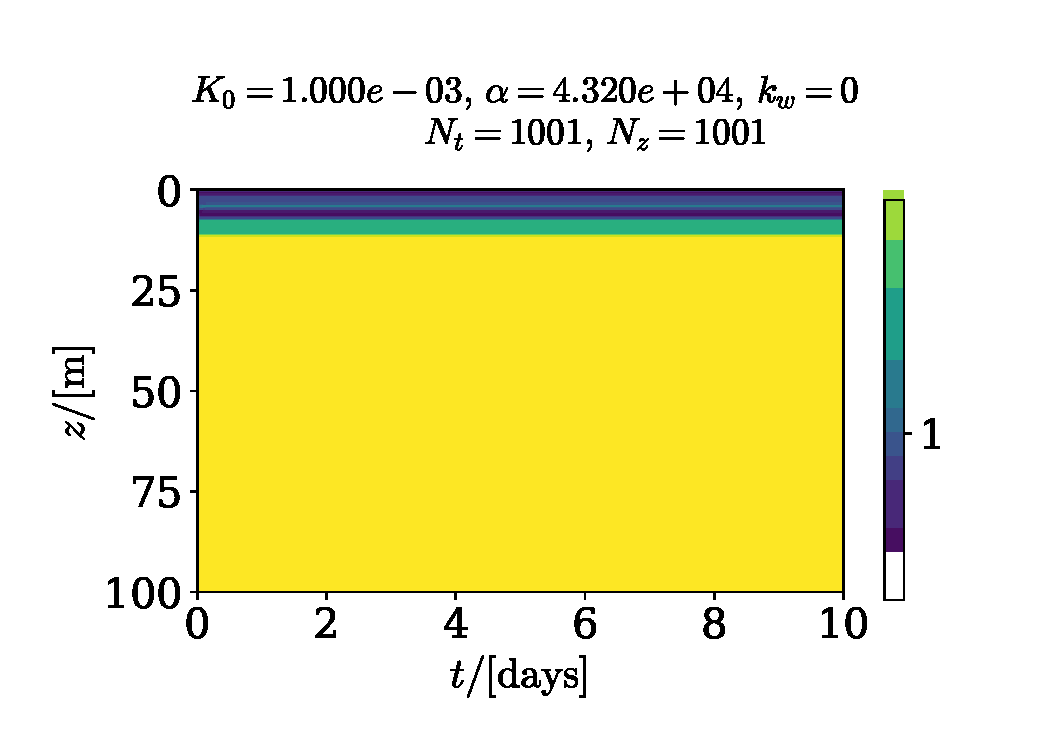
\includegraphics[width=.49\textwidth]{../plots/test1}
        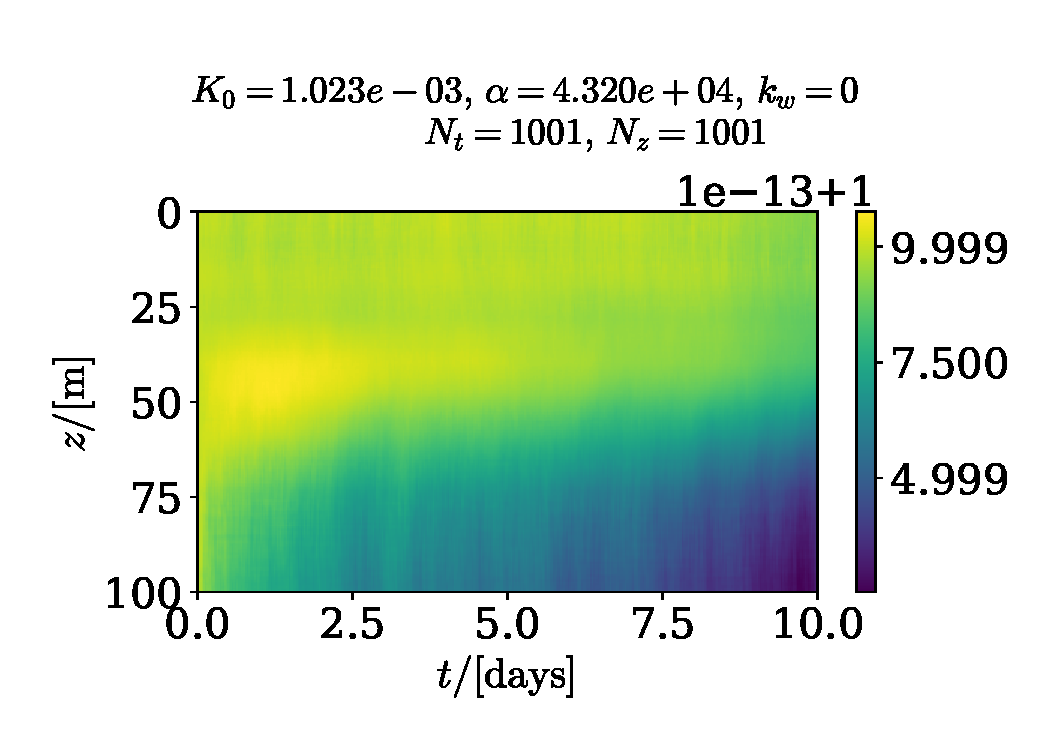
\includegraphics[width=.49\textwidth]{../plots/test1_varK}
        \label{Constant cons}
        \caption{The time evolution of an constant concentration. The system on the left has a constant $K(z)$, while system of the right has an oscillatory $K$. The largest deviation of the system is of order $10^{-11}$ and $10^{-12}$, respectively.}
    \end{figure}

    The systems should also, given $k_w=0$, conserve mass.

    \begin{figure}
        \centering
        \includegraphics[width=.49\textwidth]{../plots/test2_c}
        \includegraphics[width=.49\textwidth]{../plots/test2_m}
        \label{Consv mass}
        \caption{The evolution of a gaussian distribution of \ce{CO2} is shown on the left. On the right, the relative change in mass as a function of time is plotted. }
    \end{figure}


    \begin{figure}
        \centering
        \includegraphics[width=.49\textwidth]{../plots/conv_test}
        \label{convergence test}
        \caption{}
    \end{figure}
    \bibliography{report}
    \bibliographystyle{plain}

\end{document}